\begin{table}[h!]
	\caption{The RandomForestClassifier parameters}
	\begin{tabular}{ | l | l | p{7cm} |}
		\hline
		\textbf{Parameter} & \textbf{Default} & \textbf{Description}\\
		\hline
		$n\_estimators$ & 10 & Number of trees in the forest\\
		\hline
		$criterion$ & gini & Function to measure the quality of a split. "`gini"' for Gini impurity and "`entropy"' for information gain\\
		\hline
		$max\_depth$ & None &The maximum depth of the tree.\\
		\hline
		$max\_features$ & None & The number of features to consider when looking for the best split:\\
		\hline
	\end{tabular}
	\label{table:RFdefaults}
\end{table}
The following set of hyper-parameter values was used:\\
\begin{itemize}
	\item n\_estimators: 200
	\item criterion: ['gini', 'entropy']
	\item max\_depth: [2, 4, 6, 8],
	\item max\_features': [1.0, 0.7, 0.3, 0.1,'auto','sqrt','log2']
\end{itemize}
\subsubsection{Results}
\begin{table}[h!]
	\caption{Grid search output}
	\centering
	\begin{tabular}{ | l | c | c | c |}
		\hline
		$\bf{params_n}$ & \bf{criterion} &  \bf{mx\_features} & \bf{log\_loss} \\ \hline
		$params_1$ & 'gini' & 'auto' & 0.8646 \\ \hline
		$params_2$ & 'entropy' & 'auto' & 0.8969 \\ \hline
		$params_3$ & 'gini' & 'sqrt' & 0.9018 \\ \hline
		$params_4$ & 'gini' & 'log2' & 0.9336 \\ \hline
		$params_5$ & 'entropy' & 'log2' & 0.9635 \\ \hline
	\end{tabular}
\end{table}
The best parameters founds were selected, with exception of the number of estimators. This was varied in order to measure the performance vs the number of trees. It is important to remember that each tree in the forest is independent from one another and a large number of trees won't always imply that a better performance will be obtained even if testing over the training set.\\

Two different performance metrics were used, the LogLoss and the accuracy which as we can see in Figure \ref{fig:RFlog_loss} and Figure \ref{fig:RFaccuracy} behave differently. Accuracy is maintained relatively constant for both the training and testing set whereas the LogLoss provides us a more detailed visualization of the improvement in the predicted probabilities. Performance stops improving after 200 trees and no evident sign of overfitting is presented. If the only metric used was to be accuracy this fact couldn't be so easily seen leading to a less reliable score.\\
\begin{figure}[h!]
    \centering
    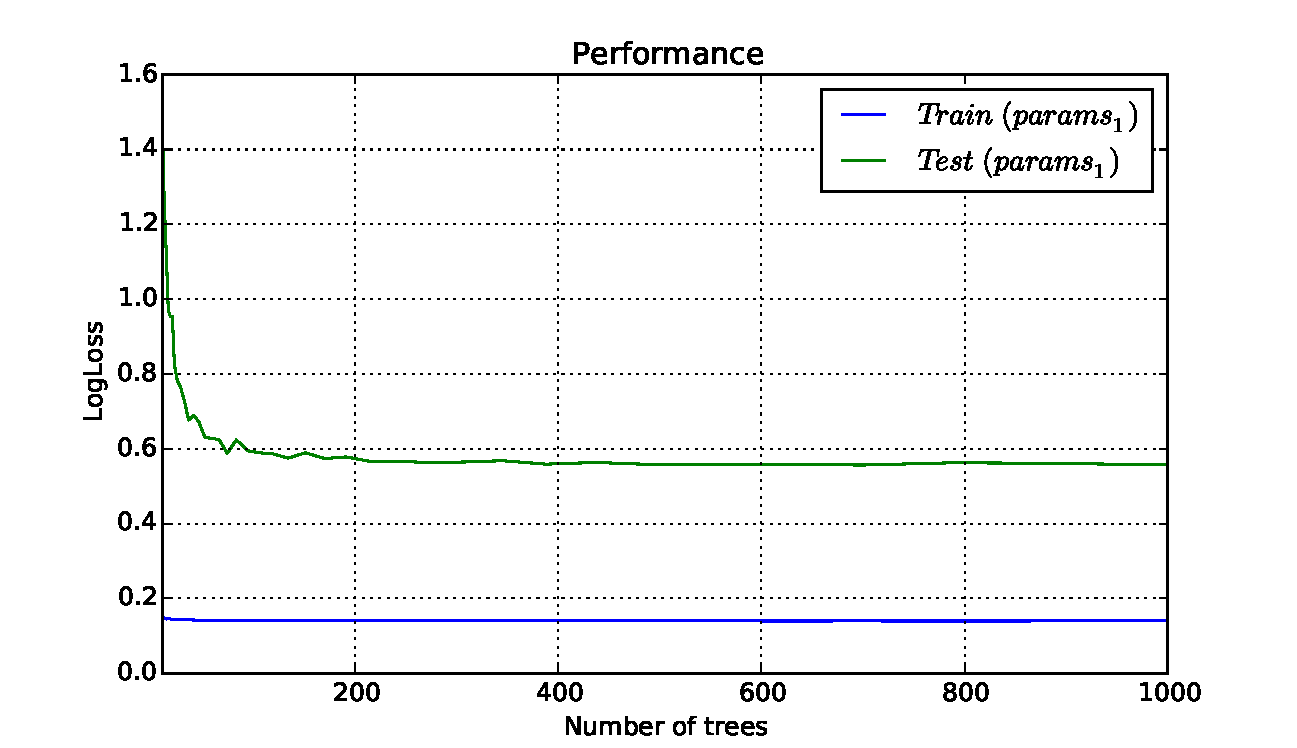
\includegraphics[width=1\textwidth]{RFlogloss}
    \caption{Performance using logarithmic loss as a metric}
    \label{fig:RFlog_loss}
\end{figure}\\
\begin{figure}[h!]
    \centering
    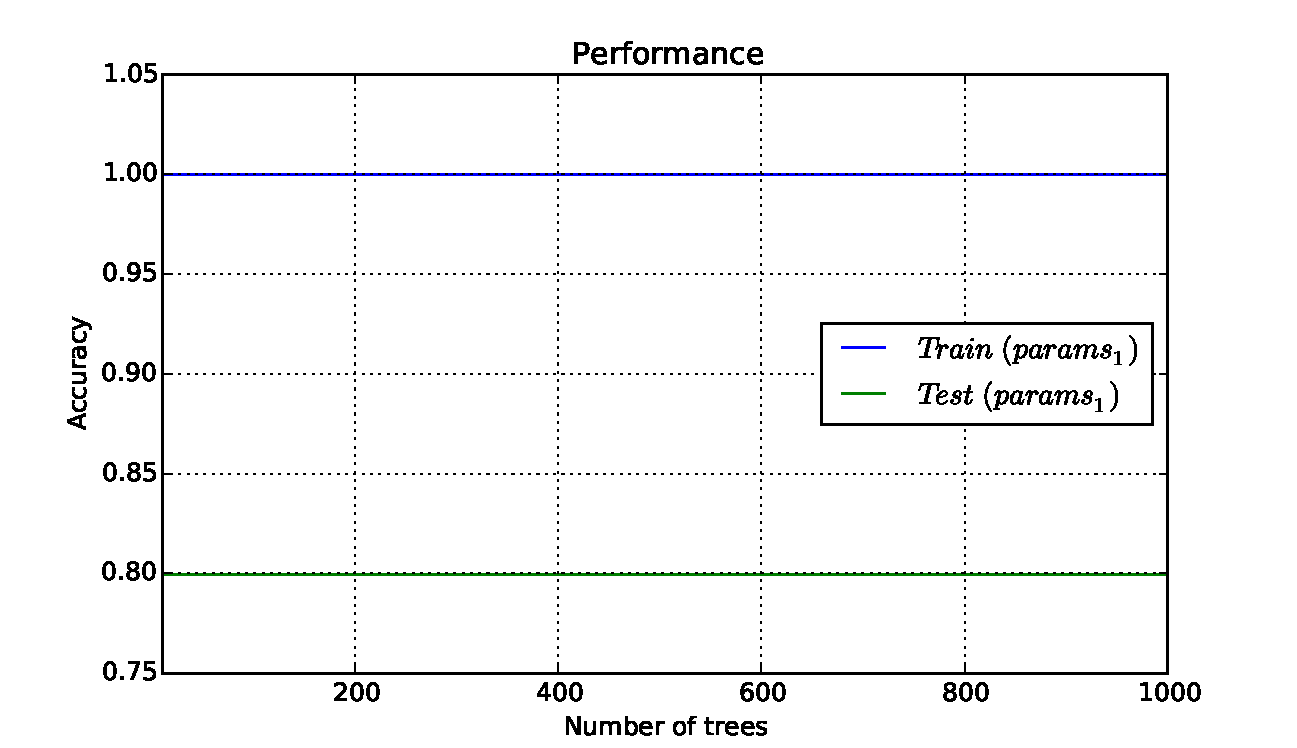
\includegraphics[width=1\textwidth]{RFaccuracy}
    \caption{Performance using accuracy as a metric}
    \label{fig:RFaccuracy}
\end{figure}\\
Confusion matrices were plotted using 400 as the number of estimators.
\begin{figure}[h!]
    \centering
    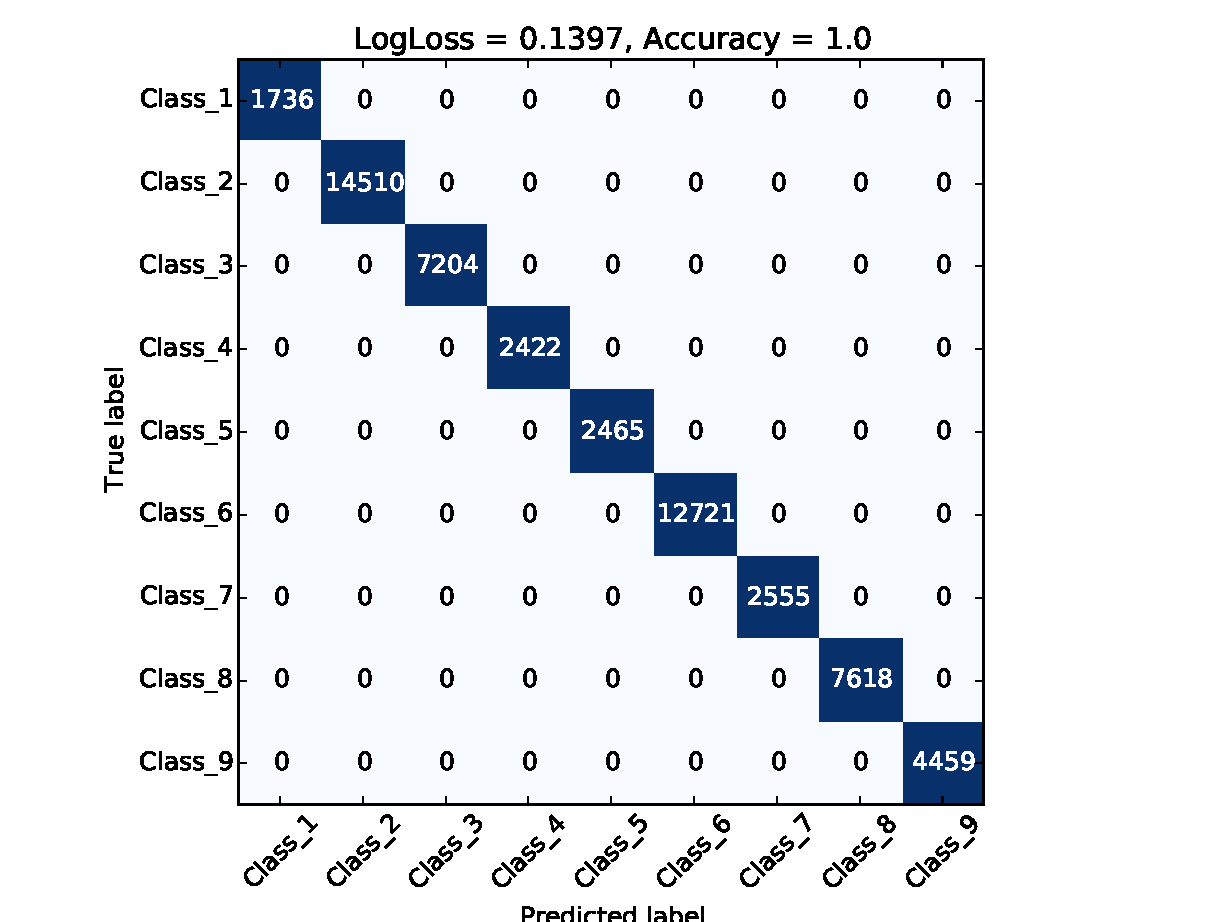
\includegraphics[width=0.7\textwidth]{RFcm_train}
    \caption{Random Forests confusion matrix using training dataset}
    \label{fig:RFcm_train}
\end{figure}
\begin{figure}[h!]
    \centering
    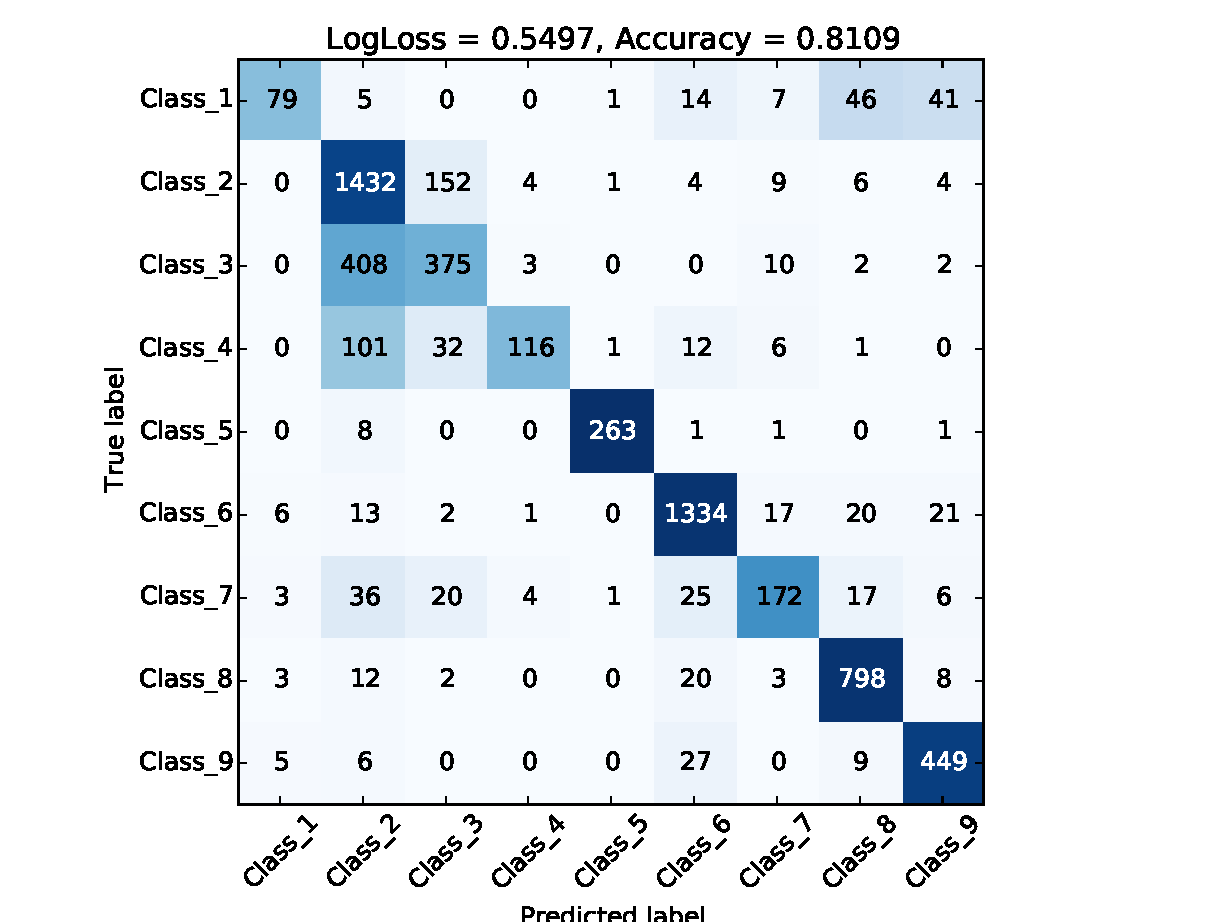
\includegraphics[width=0.7\textwidth]{RFcm_test}
    \caption{Random Forests confusion matrix using testing dataset}
    \label{fig:RFcm_test}
\end{figure}